\chapter{Appendix}

\vspace*{\fill}

\textit{Note : All code used in this thesis has been made available online via github - \url{https://github.com/sbmkvp/phd-thesis}.}

\cleardoublepage

%==============================================================================%
\section{Manual Counting}
%==============================================================================%

%-------------------------------------------------------------------------------
\subsection{Node.js App} \label{appendix:manualcount}
%-------------------------------------------------------------------------------
\vspace{1em}
\inputminted{javascript}{tools/manual-count/package.json}
\inputminted{javascript}{tools/manual-count/manualcount.js}

%-------------------------------------------------------------------------------
\subsection{Android App} \label{appendix:clicker}
%-------------------------------------------------------------------------------
\vspace{1em}
The Android manifest which defines the whole application along with the permissions it needs to function.
\inputminted{xml}{tools/clicker/manifest.xml}
\vspace{1em}
The layout of the app.
\inputminted{xml}{tools/clicker/layout.xml}
\vspace{1em}
The main logic of the app.
\inputminted{java}{tools/clicker/activity.java}
\pagebreak

%==============================================================================%
\section{Pilot Study}
%==============================================================================%

%-------------------------------------------------------------------------------
\subsection{Sensor} \label{appendix:pilot:sensor}
%-------------------------------------------------------------------------------
\vspace{1em}
\inputminted{javascript}{tools/pilot-study/sensor-package.json}
\inputminted{javascript}{tools/pilot-study/sensor-collect.js}
\inputminted{bash}{tools/pilot-study/sensor-collect.sh}

%-------------------------------------------------------------------------------
\subsection{Server} \label{appendix:pilot:server}
%-------------------------------------------------------------------------------
\vspace{1em}
\inputminted{javascript}{tools/pilot-study/server-package.json}
\inputminted{javascript}{tools/pilot-study/server-server.js}

%==============================================================================%
\section{Data Pipeline}\label{appendix:data:pipeline}
%==============================================================================%

\subsection{Sample configuration file } 
%-------------------------------------------------------------------------------
\vspace{1em}
\inputminted{javascript}{tools/pipeline/config_sample.json}

\subsection{Data Pipeline}
%-------------------------------------------------------------------------------
\vspace{1em}
\inputminted{bash}{tools/pipeline/pipeline}

\subsection{Daily Download}
%-------------------------------------------------------------------------------
\vspace{1em}
\inputminted{bash}{tools/pipeline/daily}

\subsection{Batch Download}
%-------------------------------------------------------------------------------
\vspace{1em}
\inputminted{bash}{tools/pipeline/batch}

\subsection{Component Scripts}
%-------------------------------------------------------------------------------
\vspace{1em}
Download the data from Azure data store.
\inputminted{bash}{tools/pipeline/scripts/download}
Transform the JSON files to CSV.
\inputminted{bash}{tools/pipeline/scripts/flatten}
Hash the MAC address field.
\inputminted{R}{tools/pipeline/scripts/hash}
Find the locations of the sensors.
\inputminted{bash}{tools/pipeline/scripts/locate}
Aggregate the counts based on MAC addresses.
\inputminted{R}{tools/pipeline/scripts/count}
Adjust the local counts based on probes to MAC ratio.
\inputminted{R}{tools/pipeline/scripts/adjust}
Impute missing values using Kalman filter.
\inputminted{R}{tools/pipeline/scripts/impute}
Download and update meta data.
\inputminted{bash}{tools/pipeline/scripts/meta_data}
Rotate the salt value in the configuration file.
\inputminted{bash}{tools/pipeline/scripts/rotate_salt}

\subsection{SQL queries}
%-------------------------------------------------------------------------------
\vspace{1em}
Manual counts.
\inputminted{sql}{tools/pipeline/queries/calibrations}
Device information.
\inputminted{sql}{tools/pipeline/queries/devices}
Location information.
\inputminted{sql}{tools/pipeline/queries/locations}
Installation notes.
\inputminted{sql}{tools/pipeline/queries/installs}

%==============================================================================%
\section{Benchmarking Data Tookit} \label{appendix:benchmark}
%==============================================================================%

This section documents all the code that has been used in the research.
The programming languages used are including but not limited to R, Bash, JavaScript and SQL.

%-------------------------------------------------------------------------------
\subsection{Simple implementation in R}
%-------------------------------------------------------------------------------
This R script lists all files in a given folder, parses them as JSON data serially, aggregates the records for each time interval and finally writes it to disk as a CSV file.
\vspace{1em}
\inputminted{R}{analysis/data-toolkit/old-toolkit.r}

%-------------------------------------------------------------------------------
\subsection{Serial implementation in bash}
%-------------------------------------------------------------------------------
This bash script lists all the files in a given folder, parses them into JSON data \textit{serially}, aggregates the resulting records for each time interval and finally writes it to disk as a CSV file.
\vspace{1em}
\inputminted{bash}{analysis/data-toolkit/new-toolkit.sh}

%-------------------------------------------------------------------------------
\subsection{Parallel implementation in bash}
%-------------------------------------------------------------------------------

This bash script lists all the files in a given folder, parses them into JSON data \textit{in parallel}, aggregates the resulting records for each time interval and finally writes it to disk as a CSV file.
\vspace{1em}
\inputminted{bash}{analysis/data-toolkit/new-toolkit-parallel.sh}
\pagebreak

%===============================================================================
\section{Sample Probe Request} \label{appendix:sampleprobe}
%===============================================================================
This is a sample probe request captured using tshark and saved in the JSON format.

\vspace{1em}
\inputminted{javascript}{analysis/data-collection/samplepacket.json}
\pagebreak

%==============================================================================%
\section{Open-source software used}\label{appendix:software}
%==============================================================================%

This section provides a non-exhaustive list of the key open-source/free software that have been used in this research.

\begin{itemize}
\item \textbf{R} - programming language for statistical computing
    \begin{itemize}
      \item \textbf{tidyverse} - An opinionated collection of R packages designed for data science. 
      \item \textbf{imputeTS} - Package for imputation missing values in univariate time series.
      \item \textbf{tmap} - A flexible, layer-based, and easy to use package to create thematic maps.
      \item \textbf{lubridate} - Package for working with date-times and time-spans
      \item \textbf{ggplot2} - A system for declaratively creating graphics, based on The Grammar of Graphics.
      \item \textbf{classInt} -  Package for choosing univariate class intervals for mapping or other graphics purposes.
      \item \textbf{Cairo} - 2D graphics library with support for multiple output devices.
      \item \textbf{fmsb} - Package with methods and functions for demographic analysis.
      \item \textbf{digest} - Package for the creation of hash digests of arbitrary R objects.
      \item \textbf{ggrepel} - Package that provides geoms for ggplot2 to repel overlapping text labels.
      \item \textbf{ggridges} - Package for creating ridge plots.
      \item \textbf{maptools} - Package for manipulating geographic data.
      \item \textbf{tidyquant} - Package that brings financial analysis and charting to tidyverse.
      \item \textbf{treemapify} - Package for creating tree-maps.
      \item \textbf{spatial features} - Package for manipulating geographic data within tidyverse.
      \item \textbf{RJSONIO} - Package for manipulating JSON objects.
      \item \textbf{rgdal} - Wrapper for the Geospatial Data Abstraction Library.
      \item \textbf{rgeos} - Wrapper for the Geometry Engine - Open Source.
      \item \textbf{viridis} - Package providing pretty color scales for visualisations. 
      \item \textbf{xtable} - Package for coercing data to LaTeX and HTML tables.
      \item \textbf{scales} - Package for providing graphical scales mapping data to aesthetics.
      \item \textbf{showtext} - Package for managing fonts. 
      \item \textbf{reshape2} - Package for transforming data between long and wide format.
      \item \textbf{rmarkdown} - Package for integrating markdown with R assisting reproducible research.
    \end{itemize}
  \item \textbf{Python} - An interpreted, high-level, general-purpose programming language.
  \item \textbf{PHP} - A general-purpose programming language originally designed for server-side web development.
  \item \textbf{JavaScript} - A high-level, interpreted scripting language for client-side web development.
    \begin{itemize}
      \item \textbf{node.js} - JavaScript based runtime built on chrome's V8 engine.
      \item \textbf{socket.io} - web sockets implementation for real-time, bidirectional and event-based communication.
      \item \textbf{moment.js} - JavaScript library for dealing with date-time and time-spans.
      \item \textbf{pm2} - Process management library for working with node.js applications.
      \item \textbf{express} - A fast, unopinionated, minimalist web framework for Node.js
      \item \textbf{Data Driven Documents} - A JavaScript library for visualizing data with HTML, SVG, and CSS.
      \item \textbf{jQuery} - A JavaScript library designed to simplify HTML DOM manipulation.
      \item \textbf{Bootstrap} - A framework for building responsive, mobile first websites.
      \item \textbf{highcharts} - A JavaScript library for drawing interactive charts from data.
    \end{itemize}
  \item \textbf{GNU/Linux} - An operating system and an extensive collection of open source and free computer software.
    \begin{itemize}
      \item \textbf{Arch Linux} - A lightweight and flexible Linux distribution.
      \item \textbf{CentOS} - A community supported computing platform compatible with Red Hat Enterprise Linux.
      \item \textbf{Debian} - A Linux distribution focussing on stability. 
      \item \textbf{Ubuntu} - A Debian based Linux distribution focussing on ease of use.
      \item \textbf{Alpine Linux} - Ultra minimalistic Linux distribution focussing on resource efficiency.
    \end{itemize}
  \item \textbf{git} - A simple distributed version control system.
  \item \textbf{imagemagik} - Suite for displaying, converting and editing images.
  \item \textbf{ffmpeg} - Suite for converting and editing video files.
  \item \textbf{fzf} - A general-purpose command-line fuzzy finder.
  \item \textbf{ripgrep} - Rust based grep implementation for searching the content of files.
  \item \textbf{MySQL} - A relational database management system focussing on speed and ease of use.
  \item \textbf{Postgres} - A relational database management system emphasizing extensibility and technical standards compliance.
  \item \textbf{PostGIS} - Extension providing spatial objects for the PostgreSQL database.
  \item \textbf{QGIS} - Geographic Information System for creating, editing, visualising, analysing and publishing geospatial information.
  \item \textbf{gdal} - Geographic Data abstraction library.
  \item \textbf{geos} - Geometry Engine Open Source.
  \item \textbf{igraph} - R and Python library for dealing with networks / Graphs.
  \item \textbf{OpenStreetMap} - A collaborative project to create a free editable map of the world.
  \item \textbf{Leaflet} - A JavaScript library for mobile-friendly interactive maps.
  \item \textbf{Android } - Open source mobile operating system based on Linux.
  \item \textbf{vim} - Vim is a highly configurable, modal text editor built with focus on efficient.
  \item \textbf{Latex} - A high quality professional typesetting system.
  \item \textbf{jq} - A command line based JSON processor.
  \item \textbf{Apache} - A feature rich web server.
  \item \textbf{nginx} - A asynchronous, event-driven web server focussing on resource efficiency.
  \item \textbf{OpenJDK} - An open source implementation of the Java Platform.
  \item \textbf{Wireshark} - A free and open-source packet analyzer
  \item \textbf{OpenSSH} - A connectivity tool for remote login with the SSH protocol.
  \item \textbf{OpenSSL} - A full-featured toolkit for the Transport Layer Security and Secure Sockets Layer protocols.
  \item \textbf{GNUPG} - A complete and free implementation of the OpenPGP standard.
  \item \textbf{gnu-parallel} - A shell tool for executing jobs in parallel using one or more computers.
  \item \textbf{Libreoffice} - A free and open-source office suite built by The Document Foundation.
  \item \textbf{RaspberryPi} - A series of low-cost, flexible single-board computers.
  \item \textbf{Docker} - A platform for doing OS level virtualisation for delivering software.
  \item \textbf{termux} - A terminal emulator and Linux environment for Android.
\end{itemize}

%===============================================================================
% \chapter{Research Article}
%===============================================================================
% 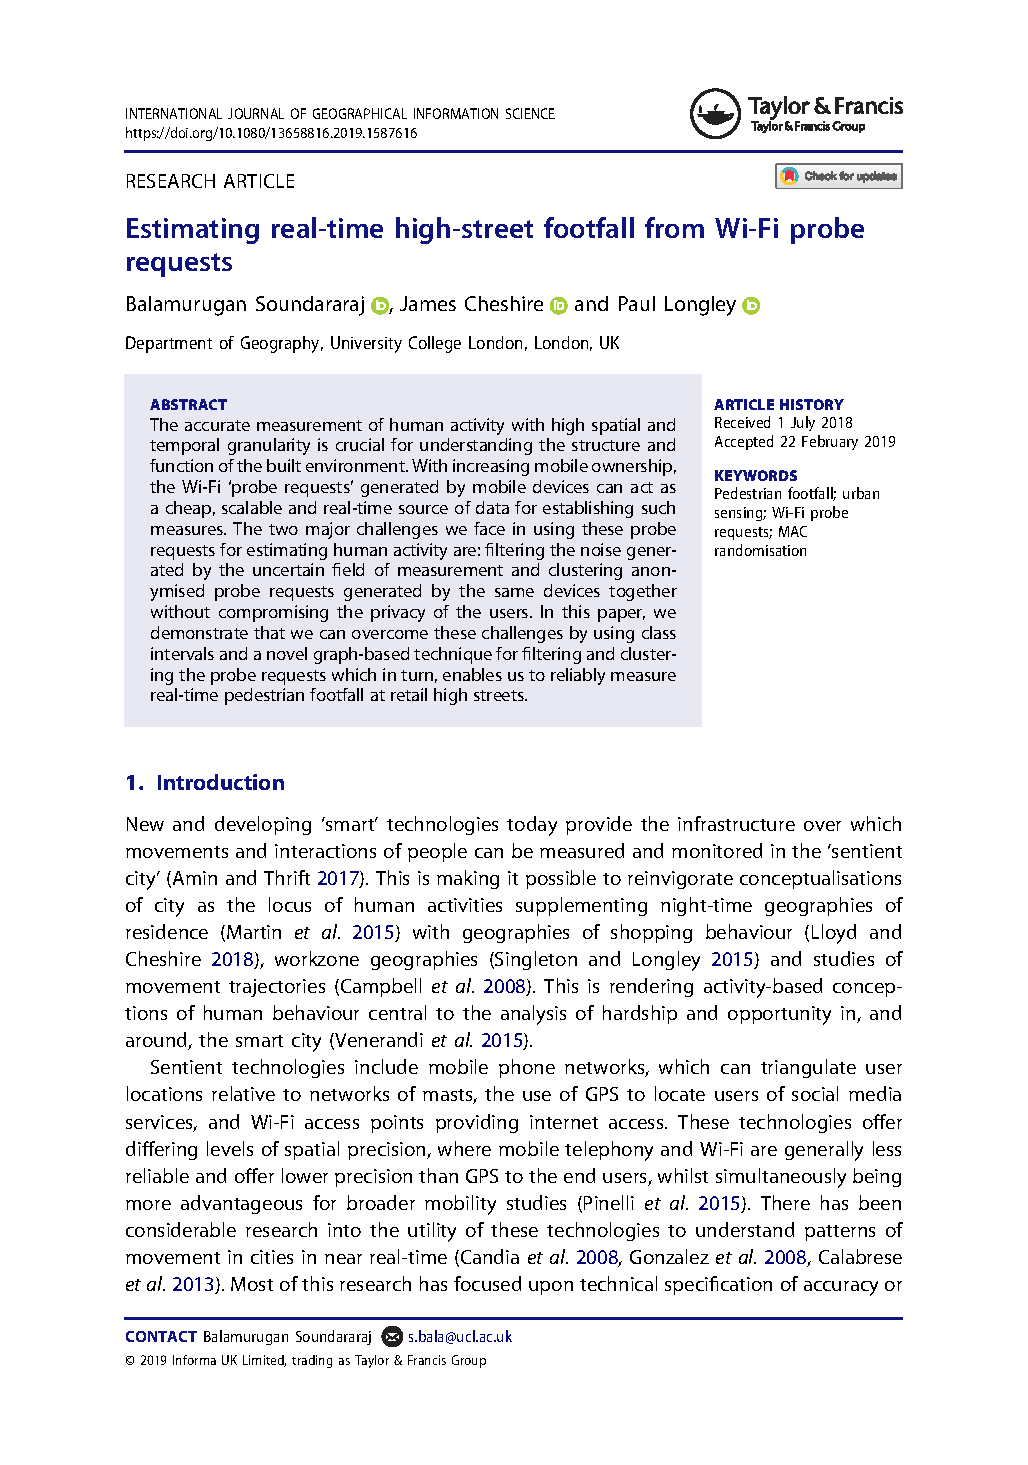
\includepdf[pages=1-15]{documents/ijgis-paper.pdf}
